\section{Les outils}
\subsection{Introduction}
\begin{frame}{Introduction}
	En C, certaines erreurs d'exécution sont très difficiles parfois même impossibles à déboguer. Que pouvons-nous faire alors? Les outils à l'aide!
	\begin{alertblock}{Exemple d'erreurs d'exécution étranges}
	\begin{itemize}
		\item \texttt{Segmentation fault (core dumped)}
		\item \texttt{*** stack smashing detected ***: terminated}
		\item \texttt{stack around the variable .. was corrupted}
		\item \texttt{memory heap corruption}
		\item \texttt{munmap\_chunk(): invalid pointer : 0x0fa1ca5a}
	\end{itemize}
	\end{alertblock}
	\begin{alertblock}{Grâce à l'outillage, nous pourrons résoudre ces problèmes !}
	\end{alertblock}
\end{frame}

\subsection{Compilateur : GCC/Clang}
\begin{frame}{Compilateur}
	\begin{itemize}
		\item Connaître le compilateur et ce qu'il peut faire est nécessaire, cela peut vous faire gagner beaucoup de temps.
		\item Il existe de nombreuses options et indicateurs du compilateur qui facilitent le débogage. 
		\item Connaître ses différentes options et comment les manipuler est nécessaire!
	\end{itemize}
\end{frame}

\begin{frame}{Compilateur}
	\begin{block}{Les flags d'optimisation :}
		\begin{itemize}
			\item \texttt{O0} : Aucune optimisation (par défaut); génère du code non optimisé mais a le temps de compilation le plus rapide.
			\item \texttt{O1} : Optimisation modérée; optimise raisonnablement bien mais ne dégrade pas le temps de compilation de manière significative.
			\item \texttt{O2} : Optimisation complète; génère du code hautement optimisé et a le temps de compilation le plus lent.
			\item \texttt{O3} : Optimisation complète comme en \texttt{-O2}; utilise aussi un \alert{inlining} automatique plus agressive et tente de vectoriser les boucles.
		\end{itemize}
	\end{block}
\end{frame}

\begin{frame}{Compilateur}
	\begin{block}{Les flags d'optimisation :}
		\begin{itemize}
			\item \texttt{Os} : Optimise l'utilisation de l'espace (code et données) du programme résultant.
			\item \texttt{Ofast} : Ne respecte pas strictement les standards. Active toutes les optimisations \texttt{-O3}. Il permet également certaines optimisations non conformes à la norme, il doit donc être utilisé avec prudence.
		\end{itemize}
	\end{block}
\end{frame}

\begin{frame}{Compilateur}
	\begin{block}{Les flags d'optimisation :}
		\begin{itemize}
			\item \texttt{Og} : Optimise l'expérience de débogage. \texttt{-Og} devrait être le niveau d'optimisation de choix pour le débogage, offrant un niveau d'optimisation raisonnable tout en maintenant une compilation rapide et une bonne expérience de débogage. C'est mieux que \texttt{-O0} pour produire du code déboguable car certaines passes du compilateur qui collectent des informations de débogage sont désactivées à \texttt{-O0}.
		\end{itemize}
	\end{block}
\end{frame}

\begin{frame}{Compilateur}
	\begin{block}{L'informations de débogage : debugging symbols}
		Pour activer la génération \alert{d'informations de débogage}, vous devez fournir \alert{\texttt{-g}} au moment de la compilation. Cet indicateur est nécessaire pour le débogage et rendra l'utilisation d'un débogueur (comme gdb) beaucoup plus facile. Il montrera exactement où l'erreur s'est produite (nom du fichier et numéro de ligne)
	\end{block}
	\begin{alertblock}{Ce qu'il faut retenir}
		Lors du \alert{débogage} du code, essayez d'utiliser \texttt{-Og} et \texttt{-g} chaque fois que c'est possible car cela facilite le débogage. Si ce n'est pas possible pour une raison quelconque, n'utilisez aucun flag \texttt{-O}. de cette façon, le compilateur adoptera par défaut \texttt{-O0}, ce qui est toujours pas mal pour le débogage.
	\end{alertblock}
\end{frame}

\begin{frame}{Compilateur}
	\framesubtitle{Autres options utiles}
	\begin{block}{Activer plus de warning}
		\begin{itemize}
			\item \alert{\texttt{-pedantic}} : Produit un avertissement lorsque les normes C ne sont pas respectées. Il produit également des avertissements lorsque des extensions non standard sont utilisées.
			\item \alert{\texttt{-Wall}} : Active tous les avertissements.
			\item \alert{\texttt{-Wextra}} : Active encore plus d'avertissements qui ne sont pas activés par \alert{\texttt{-Wall}}.
			\item \alert{\texttt{-Werror}} : Transforme tous les avertissements en erreurs.
		\end{itemize}
	\end{block}
\end{frame}

\begin{frame}{Compilateur}
	\framesubtitle{Autres options utiles}
	\begin{block}{Utilisation d'un sanatizer : \texttt{-fsanatize=option}}
		Les options peuvent être :
		\begin{itemize}
			\item \alert{\texttt{address}} : toutes sortes de fuites et de débordements peuvent être détectés avec précision, détection de niveau d'adresse, tas et pile.
			\item \alert{\texttt{leak}} : il ne détecte que les fuites et débordement mémoire au niveau du tas, mais pas la pile.
			\item \alert{\texttt{undefined}} : active un détecteur de comportement indéfini. Divers calculs sont instrumentés lors de l'exécution
			\item \alert{\texttt{all}} : active toutes les options mentionnées ci-dessus et plus \footnote[frame]{pour plus de \href{https://gcc.gnu.org/onlinedocs/gcc-5.3.0/gcc/Debugging-Options.html}{détail}}
		\end{itemize}
	\end{block}
\end{frame}

\subsection{Débogueur : GDB}
\begin{frame}{Débogueur: GDB}
	\begin{block}{Définition : }
		Un débogueur ou un outil de débogage est un programme informatique utilisé pour tester et déboguer d'autres programmes. L'utilisation principale d'un débogueur est d'exécuter le programme cible dans des conditions contrôlées qui permettent au programmeur de suivre ses opérations en cours et de surveiller les changements dans les ressources informatiques qui peuvent indiquer un code défectueux.
	\end{block}
	\begin{alertblock}{Un débogueur vous aidera à détecter les erreurs mais ne les corrigera pas à votre place. C'est le travail des programmeurs de corriger le code}
	\end{alertblock}
\end{frame}

\begin{frame}{Débogueur: GDB}
	\begin{exampleblock}{Débogueurs courants utilisés pour le langage C/C++}
		\begin{itemize}
			\item GDB : Débogueur GNU
			\item LLDB : est le composant de débogage du projet LLVM.
		\end{itemize}
	\end{exampleblock}
	\begin{alertblock}{Dans ces diapositives, nous ne couvrirons que gdb, car c'est le plus couramment utilisé. Cependant, les commandes devraient être les mêmes pour LLDB}
	\end{alertblock}
\end{frame}

\begin{frame}{Débogueur: GDB}
	\framesubtitle{Utilisation de GDB}
	\begin{enumerate}
		\item Afin d'utiliser correctement GDB, le compilateur \alert{doit} être compilé avec le flag \alert{\texttt{-g}}. Si ce n'est pas le cas, le débogueur aura du mal à trouver les noms de fichiers et les numéros de ligne. \\
		\item Après avoir compilé avec les bonnes options, vous pouvez lancer GDB en utilisant la commande : \alert{\texttt{gdb ./nom\_executable}} .\\ 
	\end{enumerate}
	Si vous voulez lancer GDB avec une interface utilisateur textuelle, utilisez l'option \alert{\texttt{-tui}}. Cette option vous permettra de voir le code source, les points d'arrêt, etc. lors du débogage.
\end{frame}

\begin{frame}{Débogueur: GDB}
	% \framesubtitle{Utilisation de GDB}
	\begin{alertblock}{Attention : }
		Si vous voyez le message suivant: \\
		\texttt{(No debugging symbols found in ...)} \\
		Ca signifie que vous n'avez pas compilé avec \texttt{-g}. Le débogage de code sera plus difficile et parfois même inutile.
	\end{alertblock}
	\begin{figure}[!h]
		\centering
		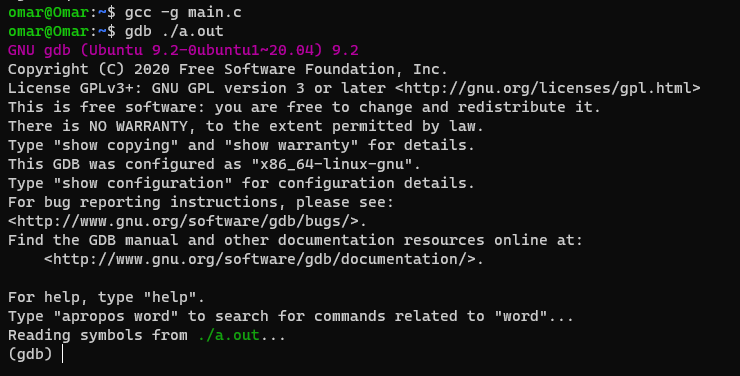
\includegraphics[width=80mm]{resources/loading_gdb}
		\caption{Un programme chargé avec succès par GDB}
	\end{figure}
\end{frame}
	
\begin{frame}{Débogueur: GDB}
	\framesubtitle{Commandes GDB}
	\begin{itemize}
		\item \alert{\texttt{file executable}} : spécifie le programme que vous souhaitez déboguer.
		\item \alert{\texttt{run}} : exécute le programme chargé. des arguments peuvent également être fournis.
		\item \alert{\texttt{list}} : afficher quelques lignes du code source.
		\item \alert{\texttt{break filename:linenumber}} : définit un point d'arrêt sur le numéro de ligne donné dans le fichier source. L'exécution s'arrêtera avant que cette ligne ne soit exécutée.
		\item \alert{\texttt{info breakpoints}} : afficher des informations sur tous les points d'arrêt, y compris son numéro.
		\item \alert{\texttt{delete id}} : supprimer le point d'arrêt numéroté \alert{\texttt{id}}
		\item \alert{\texttt{continue}} : continuera à exécuter le programme à nouveau, après l'avoir arrêté.
	\end{itemize}
\end{frame}

\begin{frame}{Débogueur: GDB}
	\framesubtitle{Commandes GDB}
	\begin{itemize}
		\item \alert{\texttt{info locals}} : Afficher toutes les variables locales
		\item \alert{\texttt{info args}} : Afficher tous les arguments de la fonction en cours d'exécution
		\item \alert{\texttt{backtrace}} : Imprime la pile d'appels jusqu'au point d'arrêt actuel. Utile pour savoir quelles fonctions sont appelées avant qu'un crash ne se produise
		\item \alert{\texttt{backtrace full}} : Comme backtrace mais affiche aussi les variables locales
		\item \alert{\texttt{print expression}} : affichera la valeur de l'expression, qui pourrait être juste un nom de variable.
		\item \alert{\texttt{set varname=value}} : change la valeur d'une variable et continue l'exécution avec la valeur modifiée.
		\item \alert{\texttt{disas}} : affiche le code assembleur de la fonction actuelle.
	\end{itemize}
\end{frame}

\begin{frame}{Débogueur: GDB}
	\framesubtitle{Commandes GDB}
	\begin{itemize}
		\item \alert{\texttt{step}} : exécutera la ligne du code courante, puis arrêtera à nouveau l'exécution avant la ligne suivante.
		\item \alert{\texttt{next}} : est similaire à "step", sauf que si la ligne qui va être exécutée est un appel de fonction, alors cet appel de fonction sera complètement exécuté avant que l'exécution ne s'arrête à nouveau.
		\item \alert{\texttt{until}} : comme \alert{\texttt{next}}, sauf que si vous êtes à la fin d'une boucle, \alert{\texttt{until}} continuera l'exécution jusqu'à ce que la fin de la boucle. Ceci est pratique si vous voulez voir ce qui se passe après une boucle, mais que vous ne voulez pas parcourir chaque itération.
		\item \alert{\texttt{finish}} : continuer l'exécution jusqu'à la fin de la fonction courante.
		\item \alert{\texttt{where}} : affiche le numéro de ligne en cours d'exécution
	\end{itemize}
\end{frame}

\subsection{Valgrind}
\begin{frame}{Détecter les fuites : Valgrind}
	\begin{block}{Qu'est-ce que Valgrind?}
		Valgrind est un outil de programmation pour le débogage de la mémoire, la détection des fuites de mémoire et le profilage.
	\end{block}
	\begin{alertblock}{Attention : }
		\begin{itemize}
			\item Comme pour GDB, pour que valgrind fonctionne correctement, votre programme doit être compilé avec l'option \alert{\texttt{-g}}.
			\item valgrind n'est pas installé par défaut. Vous devez l'installer manuellement.
		\end{itemize}
	\end{alertblock}
\end{frame}

\begin{frame}{Détecter les fuites : Valgrind}
	\framesubtitle{Guide d'utilisation}
	\begin{block}{Comment l'utiliser ?}
		Une fois que vous avez compilé votre programme dans les bonnes configurations. Utiliser Valgrind est simple. Il suffit d'utiliser la commande suivante : \\ 
		\alert{\texttt{valgrind -{}-leak-check=yes nom\_programme [[ args ]]}} \\
		Les arguments \texttt{[[ args ]]} sont facultatifs, mais si votre programme en a besoin, vous pouvez les transmettre de la manière mentionnée ci-dessus.
	\end{block}
\end{frame}

\defverbatim[colored]\valgrindExmpl{	
\begin{lstlisting}[language=C,tabsize=4]
#include <stdlib.h>
	
void toto()
{
	int* x = malloc(5 * sizeof(int));
	x[6] = 0;
}
	
int main()
{
	toto();
}
\end{lstlisting}}
\begin{frame}{Détecter les fuites : Valgrind}
	\framesubtitle{Guide d'utilisation : Exemple}
	Soit le code suivant :
	\valgrindExmpl
\end{frame}

\defverbatim[colored]\valgrindExmplSolution{	
\begin{lstlisting}[language=C,tabsize=4]
#include <stdlib.h>

void toto()
{
	int* tab = malloc(5 * sizeof(int));
	tab[6] = 0; // problem 1 : Exceeding allocated memory 
				// boundaries
			    // problem 2 : memory leak, tab is not freed
}

int main()
{
	toto();
}
\end{lstlisting}}
\begin{frame}{Détecter les fuites : Valgrind}
	\framesubtitle{Guide d'utilisation : Exemple}
	Compilation avec la commande : \texttt{gcc -g main.c} \\
	Execution du valgrind avec la commande :\\
	\texttt{valgrind -{}-leak-check=yes ./a.out}
	\begin{figure}[!h]
		\centering
		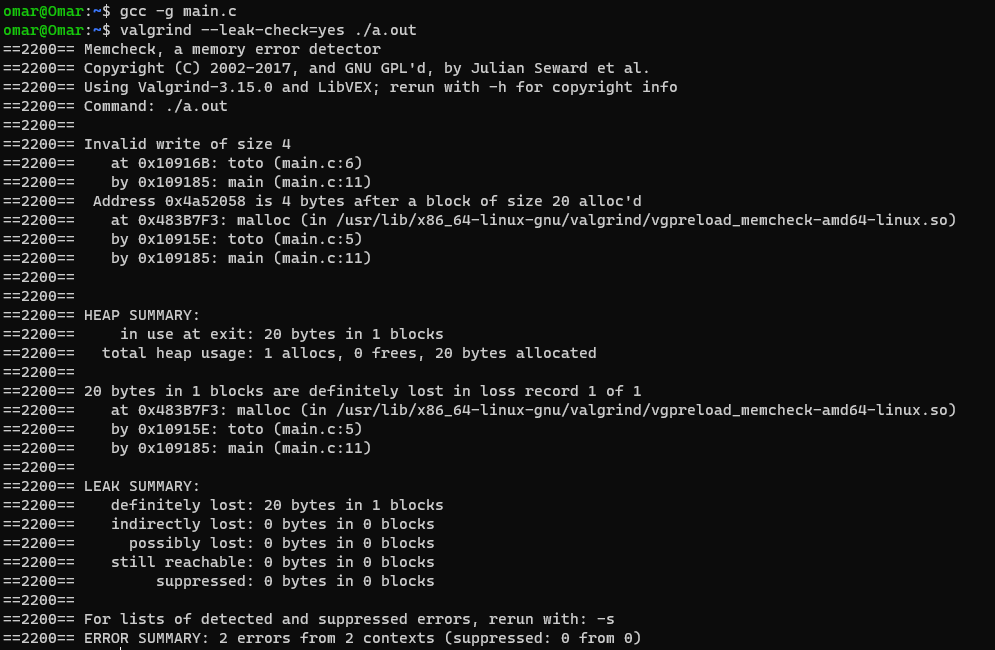
\includegraphics[width=77mm]{resources/valgrind}
		\caption{La sortie Valgrind lors de l'exécution}
	\end{figure}
\end{frame}

\defverbatim[colored]\valgrindOutputOne{	
\begin{lstlisting}[language=C,tabsize=4]
==2200== Invalid write of size 4
==2200==    at 0x10916B: toto (main.c:6)
==2200==    by 0x109185: main (main.c:11)
==2200==  Address 0x.. is 4 bytes after a block of size 20 allocd
==2200==    at 0x483B7F3: malloc (vgpreload_memcheck.so)
==2200==    by 0x10915E: toto (main.c:5)
==2200==    by 0x109185: main (main.c:11)
\end{lstlisting}}
\begin{frame}{Détecter les fuites : Valgrind}
	\framesubtitle{Comment interpréter le résultat}
	\valgrindOutputOne
\end{frame}


\begin{frame}{Détecter les fuites : Valgrind}
	\framesubtitle{Comment interpréter le résultat}
	\begin{block}{Explication : }
		- Le numéro \texttt{2200} est le PID du processus, c'est n'est pas trés important pour nous.\\
		- \alert{Ligne 1} : indique une écriture de 4 octets dans une zone mémoire qui n'appartient pas au processus. Ce qui est affiché après est la pile d'appels menant à cette erreur. \\
		- \alert{Ligne 4} : donne plus détail sur l'erreur à la ligne 1. il précise l'adresse où l'écriture s'est produite et la position de cette adresse par rapport à ce que nous avons alloué auparavant. Il montre également d'où provient cette adresse en affichant la pile d'appels.
	\end{block}
\end{frame}


\defverbatim[colored]\valgrindOutputTwo{	
\begin{lstlisting}[language=C,tabsize=4]
20 bytes in 1 blocks are definitely lost in loss record 1 of 1
   at 0x483B7F3: malloc (in vgpreload_memcheck.so)
   by 0x10915E: toto (main.c:5)
   by 0x109185: main (main.c:11)
\end{lstlisting}}
\begin{frame}{Détecter les fuites : Valgrind}
	\framesubtitle{Comment interpréter le résultat}
	\valgrindOutputTwo
	\begin{block}{Explication : }
		- \alert{Ligne 1} : indique qu'il y a un fuite de mémoire de \texttt{20} octets qui sont définitivement perdu. Les lignes juste après montrent la pile d'appels qui indique où la mémoire perdu a été allouée. \\
		- Malheureusement, Valgrind ne peut pas vous dire \alert{pourquoi} la mémoire a fui.
	\end{block}
\end{frame}

\begin{frame}{Détecter les fuites : Valgrind}
	\begin{alertblock}{ATTENTION : }
		- En fait, valgrind étant un framework, il peut faire plus que simplement détecter les fuites. Il fournit une suite d'outils et les outils que nous utilisons jusqu'à présent s'appellent \alert{Memcheck}. \\
		- \alert{Memcheck} n'est pas parfait; il produit parfois de faux positifs, et il existe des mécanismes pour supprimer ces effets secondaires. Cependant, il est généralement correct 99\% du temps, vous devez donc éviter \alert{d'ignorer} ses messages d'erreur.\\
		- \alert{Memcheck} ne peut pas détecter toutes les erreurs de mémoire. Par exemple, il ne peut pas détecter les lectures ou écritures hors limites dans des tableaux alloués statiquement sur la pile. Mais il devrait détecter de nombreuses erreurs qui pourraient planter le programme (par exemple, les erreurs de segmentation).
	\end{alertblock}
\end{frame}

\begin{frame}{Valgrind}
	\framesubtitle{Détecter la mémoire non initialisée}
	\begin{block}{Que peut-il faire d'autre pour nous?}
		Valgrind signale également les utilisations de valeurs \alert{non initialisées}, le plus souvent avec le message "Le saut ou le déplacement conditionnel dépend de la ou des valeurs non initialisées". \\
		Il peut être difficile de déterminer la cause de ces erreurs. Essayez d'utiliser \alert{\texttt{-{}-track-origins=yes}} pour obtenir des informations supplémentaires.
	\end{block}
\end{frame}

\begin{frame}{Valgrind}
	\framesubtitle{Valgrind : Au-delà de la vérification de la mémoire}
	Comme mentionné précédemment, Valgrind peut fournir un ensemble de services qui sortent du cadre de ce cours, nous ne les couvrirons donc pas ici. Parmi ces outils, on retrouve :
	\begin{itemize}
		\item \alert{\texttt{Massif}} : un profileur de tas, mesure l'utilisation de la mémoire du tas au fil du temps.
		\item \alert{\texttt{Cachegrind}} : un profileur de cache, mesurer les succès et les échecs du cache et éventuellement les prédictions de branche.
		\item \alert{\texttt{Callgrind}} : outil de profilage qui enregistre l'historique des appels des fonctions d'un programme sous forme d'un graphe.
		\item \alert{\texttt{Helgrind }} : détecte les conditions de concurrence dans le code multithread.
	\end{itemize}
\end{frame}
